% ****** Start of file apssamp.tex ******
%
%   This file is part of the APS files in the REVTeX 4.2 distribution.
%   Version 4.2a of REVTeX, December 2014
%
%   Copyright (c) 2014 The American Physical Society.
%
%   See the REVTeX 4 README file for restrictions and more information.
%
% TeX'ing this file requires that you have AMS-LaTeX 2.0 installed
% as well as the rest of the prerequisites for REVTeX 4.2
%
% See the REVTeX 4 README file
% It also requires running BibTeX. The commands are as follows:
%
%  1)  latex apssamp.tex
%  2)  bibtex apssamp
%  3)  latex apssamp.tex
%  4)  latex apssamp.tex
%

\documentclass[%
reprint,
%superscriptaddress,
%groupedaddress,
%unsortedaddress,
%runinaddress,
%frontmatterverbose, 
% preprint,
%preprintnumbers,
%nofootinbib,
%nobibnotes,
%bibnotes,
 amsmath,amssymb,
 aps,
%pra,
%prb,
%rmp,
%prstab,
%prstper,
%floatfix,
]{revtex4-2}

\usepackage{lipsum}
\usepackage{graphics}% Include figure files
\usepackage{dcolumn}% Align table columns on decimal point
\usepackage{bm}% bold math
\usepackage{hyperref}% add hypertext capabilities
%\usepackage[mathlines]{lineno}% Enable numbering of text and display math
%\linenumbers\relax % Commence numbering lines
\usepackage[inline]{asymptote}
\usepackage{svg}
\usepackage{chemformula}


%\usepackage[showframe,%Uncomment any one of the following lines to test 
%scale=0.7, marginratio={1:1, 2:3}, ignoreall,% default settings
%text={7in,10in},centering,
%margin=1.5in,
%total={6.5in,8.75in}, top=1.2in, left=0.9in, includefoot,
%height=10in,a5paper,hmargin={3cm,0.8in},
%]{geometry}

\begin{document}

\preprint{APS/123-QED}

\title{Topological Insulators} 

\author{Pierre-Antoine Graham}
\author{Jean-Baptiste Bertrand}

\altaffiliation{Physics Department, Sherbrooke University.}

\date{\today}

\begin{abstract}
The field of topological insulators is a recent and very broad. This review aims to be an introduction to the topic. It covers the basic topological concept required to understand the theory such as the idea of topological equivalence, Kramer's theorem and the berry phase. Some of the earliest and simplest application of the theory  are quickly explained. These cover the Integer Quantum and Quantum Spin Hall effect, and the example of the HGTE/CDTE heterostructure.
\end{abstract}

\maketitle

\tableofcontents

%\listoffigures


\section{\label{sec:intro} Introduction}
One of the earliest breakthrews allowed by quantum mechanics is the descritpion of metals and insulators with band theory \cite{hoddeson_development_1987} which saw light in 1930. This theory brought a microscopic understanding of the distinction between these two classes of materials and led to incredible technological advances such as the discovery of the transistor by John Bardeen and Walter Brattain in 1947 \cite{brinkman_history_1997}. Beyond its incredible success,  band theory rapidly came in contact with a myriad of intriguing quantum mechanical effects such as the integer quantum Hall effect discovered in 1980 \cite{klitzing_new_1980}. In 1982, Thouless et al. \cite{cayssol_topological_2021} figured out the topological nature of the effect and, in terms, brought topology closer to band theory. Although the integer quantum Hall effect (QH) requires a strong external magnetic field, it was theorized in 2005 by Charles Kane and Eugene Mele \cite{kane_quantum_2005} that similar topological properties could be intrinsically realized  through the quantum spin Hall effect (QSH) \cite{qi_quantum_2010}. Experiments then showed, in 2007 \cite{koenig_quantum_2007},that HgTe/CdTe
quantum wells (mercury telluride heterostructure) could produce a QSH effect. The theory and experiment of QSH effect led to a deeper classification of solids with topological band theory \cite{soluyanov_topological_nodate}. When applied to insulators, the upgraded band theory creates a separation between the trivial and the \textit{topological insulators} (TI). The latter is generally characterized by a metallic boundary and an insulating bulk \cite{moore_birth_2010} as opposed to trivial insulators which are insulating everywhere. The present review will focus on basic properties of time reversal symmetric topological insulators based on the mercury telluride example. Sec.\ref{sec:kramers} presents an overview of important ideas from topological band theory. In sec.\ref{sec:QSH}, the main properties of the QSH state are given and compared to the QH effect. Finally, a model of HgTe/CdTe
quantum is studied in sec. \ref{sec:ti_exemples}. 

\section{\label{sec:kramers} Element of topological band theory}
This sections aims to describe the notion of topological invariant and its consequence on the band structure. 
\subsection{Topological equivalence of insulators \label{subsec:Top_Band}}
In a periodic lattice potential, electrons are described by bloch states $\ket{n, \mathbf{k}}$ where $n$ is a dicrete quantum number and $\mathbf{k}$ is the crystal momentum in the brillouin zone \cite{girvin_modern_2019}. Each of those states is associated to an energy $E_{n, \mathbf{k}}$.  As it varies with $\mathbf{k}$, the energy sweeps a continous range called a band labeled with the number $n$. Bands are often separated by energy gaps where there are no associated states. Trivial insulators have a gapped ground state meaning that low energy excitations are forbidden by the presence of the gap. On the contrary, topological insulators have metallic (gapless) edge states\cite{kane_topological_2013} and are different from trivial insulators in a fundamental way. By definition, edge states are states that are exponentially localised near the edges of the sample \cite{asboth_short_2016}. Usually, the bulk of the crystal is studied under periodic boundary conditions and the edge states are neglected in the analysis. A deep principle called \textit{bulk boundary correspondance} relates the edge states to the spectrum of the bulk system \cite{kush_bulk-edge_nodate}. \\ 


The adiabatic theorem tells us that sufficiently slow modifications of the hamiltonian of a trivial insulator will change its band structure while leaving it in its ground state\cite{born_beweis_1928}. This \textit{deformation} is said to yield equivalent insulators if the gap doesn't close \cite{kane_topological_2013}. This equivalence is topological in the same way the continuous disformation from a torus to a coffee mug is. Just like the coffee mug cannot be continuously deformed into a sphere, a trivial insulator cannot be continuously \textit{deformed} into a topological insulator.\\

% For the coffee mug and the sphere, a number tells if there is topological equivalence or not.
A coffee mug and a sphere are considered topologicaly different because they do not have the same number of holes, meaning you can't smoothly deform one into the other. 
This number (of holes) is called the genus and it as analogues for topological insulators \cite{batra_physics_2020}. The central property of genus is that it only changes when the torus is broken into a sphere in a necessarly discontinuous way. %Therefore, the genus is a topological invariant for the sphere and torus.
For the QHE the relevant topological invariant %indicating the persistance of the edge states 
(under deformation of the Hamiltonian) is the Chern number. For the QSH effect, a $\mathbb{Z}_2$ invariant is involved \cite{kane_topological_2013}. In the following section, the link between time reversal symmetry and this last invariant is detailed.  Mixing symmetry, topological invariants and dimensionnality allows for a classification of topological insulators in a sort of \textit{periodic table} \cite{hasan_topological_2010}. 

\subsection{Time reversal symmetry}
In a quantum mechanical setting, an operator $U$ (unitary or anti-unitary) corresponds to a symmetry of a system when $U H U^{-1} = H$ where $H$ is the hamiltonian governing the motion of the system. For a time reversal symetric (TRS) system this means that evolution follows the same equations of motion as a movie of itself set on rewind \cite{shankar_topological_2018}. The operator sending a system to its time reverse is an anti-unitary operator noted $\Theta$ and Hamiltonians of TRS follow the relation $\Theta H \Theta^{-1} = H$. In position representation, the intuitive effects of this time reversal operator on the observables required to describe electrons (namely the spin, momentum and position observables), are the following \cite{shankar_topological_2018} : 
\begin{align*}
    \Theta \mathbf{s} \Theta^{-1} &=-\mathbf{s}, \\
    \Theta \mathbf{r} \Theta^{-1} &=\mathbf{r}, \\
    \Theta (-i\hbar\nabla) \Theta^{-1} &=+i\hbar\nabla
\end{align*}
meaning it sets electrons spinning backwards with a reversed velocity. The operator satisfying all those porperties is $\Theta = i s_y K$ where $K$ represents complex conjugation and the $i s_y$ factor ensures spin is fully reversed \cite{bernevig_topological_2013}. The essential property of the time reversal operator for electrons is that is satsifies $\Theta^2 = -1$. Hence reversing time twice for spin $1/2$ particles isn't the identity \cite{hasan_topological_2010}! This leads to Kramer's theorem which is said to be the most important theorem for time reversal invariant two dimensionnal topological insultors \cite{bernevig_topological_2013}. It states the following:\\

\fbox{\begin{minipage}{22em}
    \textbf{\underline{Kramer's Theorem}: }


    \quad For a time reversal invariant system containing an odd number of spin $1/2$ particles, there are at least two degenerate energy states \cite{bernevig_topological_2013}.
\end{minipage}}\\[0.3cm]

\begin{figure*}[!h]
    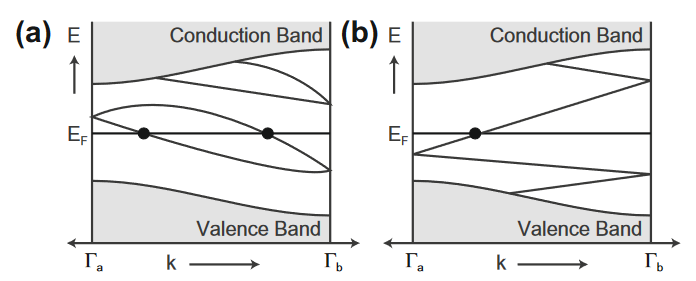
\includegraphics[scale = 0.8]{sections/visuel/kramer.png}
    \caption{Schematic representation of the two typical ways Kramer's theorem can be satisfied between TRIM points. (A) Shows a way to connect TRIM points without closing the gap. In this case there is an even amount of intersection points with the Fermi level. (B) Shows second way to connect TRIM points that closes the gap and has an odd number of intersections with the Fermi level \cite{kane_topological_2013}. To get a complete picture, on must keep in mind that the energies at $-\mathbf{k}$ are the same as the represented ones along the $k$ values of interest (they are Kramer degenerate).}
    \label{TRIM}
\end{figure*}

To use this theorem here, it must be applied to the periodic bloch states $\ket{n, \mathbf{k}}$ mentionned before. By bloch's theorem \cite{girvin_modern_2019}, these states can be written as the direct product $\ket{u_n(\mathbf{k})}\otimes \ket{\mathbf{k}}$ where $\ket{\mathbf{k}}$ takes care of the tranlsationnal symmetry of the crystal lattice and $\ket{u_n(\mathbf{k})}$ contains the details of the state over a unit cell. The basic idea of Kramers theoerem is that provided a state $\ket{u_n(\mathbf{k})}$, the action of the time reversal on it gives a state $\Theta\ket{u_n(\mathbf{k})}$ which has the same eigen energy as the first (if the hamiltonian is time reversal symmetric). Then, if there is no degeneracy the generated state must be related to the first one with a constant $c$ by $\Theta \ket{u_n(\mathbf{k})} = c \ket{u_n(\mathbf{k})}$ or else two physically different states would have the same energy\cite{kane_topological_2013}. Applying time reversal again yields
\begin{align*} 
    -\ket{u_n(\mathbf{k})} &= \Theta \{\Theta\ket{u_n(\mathbf{k})}\}\\ &= c^\star \Theta \ket{u_n(\mathbf{k})}\\ &= c c^\star \ket{u_n(\mathbf{k})}\\ &= |c|^2\ket{u_n(\mathbf{k})}
\end{align*}
where $c$ gets conjugated by $K$ and the porperty $\Theta^2 =-1$ was used. This series of equalities suggests that, if a state is non degenerate, $|c|^2 = -1$ which is impossible and leads to a contradtiction: the states must be twofold degenerate \cite{kane_topological_2013}. This can be made more precise by noting that the time reverse of $\ket{u_n(\mathbf{k})}$ is $\ket{u_{n'}(\mathbf{-k})}$ \cite{bernevig_topological_2013} (a state with reversed crystal momentum possibly living on a different band). Furthermore, the time reversed state also has reversed spin \cite{kruthoff_topology_2019}.\\

Special points called time reversal invariant momentas (TRIM) lead to a crucial effect of the theorem. They are points in the Brillouin zone that are sent to points with an equivalent cristal momentum by time reversal ($\mathbf{k} \equiv -\mathbf{k}$) \cite{kruthoff_topology_2019}. At TRIM points, the Kramer degeneracy can only be satisfied if the states come from $2$ defferent bands having different spins \cite{kruthoff_topology_2019}. This forces bands to touch at special points and then split as $\mathbf{k}$ varies trough the effect of spin orbit coupling \cite{kane_topological_2013}. In two dimensions, if there are edge states locked inside the gap of the bulk of an insulator, Kramer's theorem forces them to have one of two topologies represented on fig. \ref{TRIM} \cite{kane_topological_2013}. Consider the points having cristal momentum norm $k = 0$ ($\Gamma_a$) and the point $k = \pi/a$ ($\Gamma_b$) (with $a$ being the unit cell size in one direction): they are both TRIM points because $\mathbf{0} = - \mathbf{0}$ and $k = \pi/a$ is equivalent to $k = -\pi/a$. The edge states at the TRIM points must connect two bands by Kramer's theorem. They can either do it in a gapped way (see fig. \ref{TRIM} (A)) or in a metallic gapless way (see fig. \ref{TRIM} (B)).\\

While the band configuration in fig. \ref{TRIM} (A) can be gapped out by the addition of disorder (time reversal symmetric impurities \cite{asboth_short_2016}), configuration (B) always remain gapless and its metallic behavior is robust to deformations of the system (and of its Hamiltonian) \cite{cayssol_topological_2021}. This is where the word \textit{topological} insulator gets its meaning. To be more precise, disforming the band structure from $(A)$ to $(B)$ would requier closing the bulk gap or breaking TRS which would indicate a topological phase transition \cite{cayssol_topological_2021}. Just like it was mentionned in sec. \ref{subsec:Top_Band}, there is a number distinguishing between configuration (A) and (B) refered to as the $\mathbb{Z}_2$ topological invariant.\\

Since there are \textit{two} different ways to connect TRIM points, the invariant used to qualify the topology of a 2D TRS topological insulators is an integer $\nu$ taking values $0$ or $1$ \cite{bernevig_topological_2013}. If $\nu = 0$ then the band insulator is trivial and, if $\nu = 1$, it is topological \cite{cayssol_topological_2021}. To give precise meaning to this number, it suffice to use the notion of a \textit{Kramer pair}. Two states related to each other by the application of $\Theta$ are called a Kramer pair \cite{asboth_short_2016}. In fig. \ref{TRIM}, only one member of each Kramer pair is shown so it is important to Keep in mind that all points show effectively count for one pair. The $\nu$ invariant corresponds to the parity of the number of kramer pairs at a fixed energy \cite{asboth_short_2016}. If the number of pairs is even (A) then $\nu = 0$, the insulator is gapped and trivial. Otherwise the number of pairs is always odd (B) and the insulator is topological.

\subsection{Berry phase}
Another important concept of topological band theory is the berry phase. To define it, consider a closed $\mathbf{k}$-path in the brillouin zone. Each point of the path corresponds to a state $|u_n(\mathbf{k})\rangle$ \cite{bernevig_topological_2013} of a given band. Normally, trough the passage of time eigenstates of the hamiltonian pick up a dynamical phase depending on their associated energy. In topological systems, a new phase comes into play. Suppose, the state of the system is varied slowly on the $\mathbf{k}$-path such that the adiabatic theorem ensures that it stays in a state $|u(\mathbf{k})\rangle$ at each point. After traveling along the entire closed loop, the state has gained a global phase factor. While a part of this phase is dynamical, there is an additionnal geometrical phase $\gamma_n$ called the berry phase \cite{bernevig_topological_2013}. A \textit{parallel} (pun intended) can seen from the field of three-dimensionnal surfaces \cite{chang_x_nodate}. A vector lying on a surface is \textit{parallel transported} on  a curve of this surface if it is locally parallel to itself everywhere on the curve. If the curve happens to be a closed loop, the initial vector can be compared to a parallel transported version of itself. The angle difference between these two vectors is called the alholonomy \cite{chang_x_nodate} and is the equivalent of the berry phase. With the Gauss-Bonet theorem from differential geometry \cite{chang_x_nodate}, it is possible to relate the anholonomy to the curvature on the surface enclosed by the loop. Similarly the berry phase associated to a loop $C$ can be computed from the integral of the berry curvature $F$ on the surface $S$ enclosed by this loop in the brillouin zone \cite{kane_topological_2013}:
\begin{align*}
   \gamma_n(C) =  \int_S F \; \text{d}^2\mathbf{k}.
\end{align*}
Following the analogy with the Gauss-Bonet theorem, if the integral runs over the entire brillouin zone, it yields a topological quantity caracterizing the band $n$. The sum of these topological quantities for all filled bands is the Chern number \cite{bernevig_topological_2013}. For a three dimensionnal surface, the topological invariant is the genus of the surface like it was mentionned in sec. \ref{subsec:Top_Band}. 
%Time reversal symmetry (TRS) plays an important role in QSH topological insulators: it protects the gapless edge states \cite{kane_topological_2013}. While the QH effect requiers a magnetic field to occur (breaking of TRS), the QSH effect doesn't and it preserves TRS\cite{cayssol_topological_2021}. 


%As a global phase doesn't change the physical state of a quantum system, each state in the band structure can be multiplied by a phase factor $ e^{i \phi(\mathbf{k})}$ possibly depending on $\mathbf{k}$. This establishes the correspondance $|u(\mathbf{k})\rangle \rightarrow e^{i \phi(\mathbf{k})}|u(\mathbf{k})\rangle$ \cite{kane_topological_2013}
%\begin{enumerate}
%    \item Definition of the time reversal operator.
%    \item Description of the relation between pairs of opposite Bloch momentum in the Brillouin zone for time reversal symmetric systems.
%    \item Introduction of the notion of a Kramer pair of Bloch states and of time reversal invariant momenta. 
%    \item Summary of the main consequences of the existence of time reversal moments on the band structure. (Topology of edge modes)\\[0.5cm]
%\end{enumerate}

\section{\label{sec:QSH} Hall Effects}
One of the defining properties of topological insulators is the presence of conducting edge states with an insulating bulk. The example considered here in sec. \ref{sec:ti_exemples} is a two dimensionnal material and its edge is therefore one-dimensionnal. The QH and QSH effects both involve one-dimensionnal conduction. In one dimension, electrons can only either move forward of backward on the edge of the sample and this restriction is central for Hall effects. \cite{qi_quantum_2010}. 
\subsection{QH}
The QH effect occurs in two dimensionnal semiconductor electron gas with a strong applied magnetic field \cite{qi_quantum_2010}. It is robust to the addition of impurities in a topological way because the conducting edge states only carry current in one direction on a given side of the sample. Adding an impurity can't lead to backscattering of the electrons because there are simply no backward moving states they can scatter into \cite{qi_quantum_2010}. 

\begin{figure}[h]
    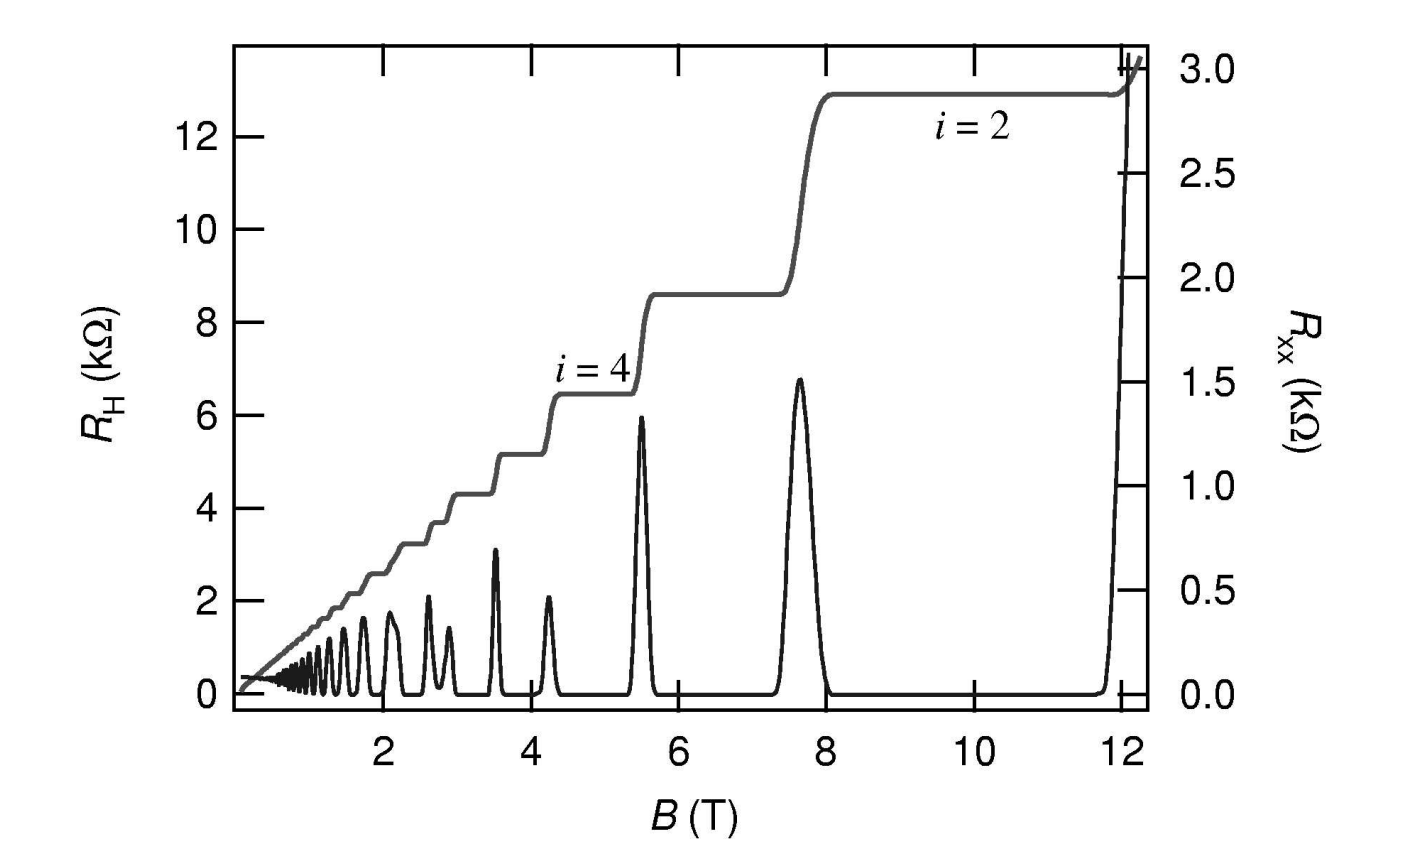
\includegraphics[width=\columnwidth]{sections/visuel/Hall_effect.png}
    \caption{Hall Effect mersurments. The upper curve represent the Hall resistance ($R_h \propto \frac{1}{\sigma_{xy}}$) and shows its plateaus while the lower one represent $R_{xx} \propto \rho_{xx}$ and shows its vanishing. Both curve are a function of the magnetic feild. \cite{jeckelmann_quantum_nodate}}
    \label{fig:Hall_effet}
\end{figure}

The QH effect consists of a two simultanious and related phenomena. The quantized \textit{Hall conductivity} $\sigma_{xy}(=\frac{I_x}{V_y})$ and the vanishing of the $\rho_{xx}$ resistivity in a 2D electron gas. The link with topology is fairly direct since the Hall Conductivity is directly proportional to the Chern number! In fact we have.
\begin{equation}
\sigma_{xy} = \mathcal{C}\frac{e^2}{\hbar}
\end{equation}

where $\mathcal{C} \in \mathbb{N}$ is the Chern number.

\begin{figure}[h!]
    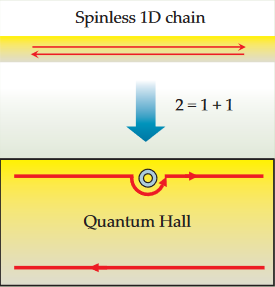
\includegraphics[scale = 0.7]{sections/visuel/spinless.png}
    \caption{Schematic representation of the conduction chanels in a spinless quantum Hall system.\cite{qi_quantum_2010}}
    \label{spinless}
\end{figure}



\subsubsection{Chern number}

% The Chern number is a topological invariant closely related to the Euler characteristic. In fact you can write the \textit{topological solid} equivalent of the \textit{Gauss-bonnet} theorem 



\subsubsection{Impossiblity of backscattering}

\subsubsection{In which material does it happen}


\subsection{QSH}

The QSH state can be obtained from the combination of two copies of the QH state \cite{buhmann_quantum_2011}. In this new state, two counter propagating channels of edge states exist on each side of the sample. Kramer's theorem (see sec. \ref{TRS}) relates these pairs of edge states with TRS \cite{buhmann_quantum_2011}. Since these states are related by TRS, they have oposite crystal momentum $\mathbf{k}$ and spin: they are \textit{helical} edge states \cite{bernevig_topological_2013}. Since helical states couple $\mathbf{k}$ with spin, QSH states can only be realised in systems with strong spi-orbit coupling \cite{qi_quantum_2010}. The number of Kramer pairs of edge states is an exemple of a $\mathbb{Z}_2$ invariant which tells if the state is topological or not \cite{koenig_quantum_2008}. Here, the helical states come in one Kramer pair (taking effect on both sides of the sample), so there is an odd number of Kramer pairs and the $\mathbb{Z}_2$ invariant allows to call the QSH state a topological state of matter.\\

The impossiblity of backscattering on impurities in the QSH state can be directly related to the effect of an antireflection lens \cite{qi_quantum_2010}. The effect of scattering on an impurity is represented in fig. \ref{lens} (B). Two quantum paths can be taken by the electron encountering the impurity. In both cases an helical state must be converted into its Kramer partner by the scattering in order to reverse the direction of its motion. When the electron goes around the impurity, its spin turns by an angle of $\pm \pi$ depending on the sens of rotation around the impurity (fig. \ref{lens} (B) up and down show the two possible paths sawpping momentum direction). The global angle difference between the two spin rotations is $2\pi$. Because the phase of half integer particles rotates with half the speed of the actual rotation whitnessed by the electron, the $2\pi$ angle difference becomes a $\pi$ phase shift. A completely destructive interference between the two quantum paths emerges and the backscattering is forbidden. This is just like perfect transmission of an antireflection lens generated by the destructive interference of the red and blue paths of fig. \ref{lens} (A). 

\begin{figure*}
    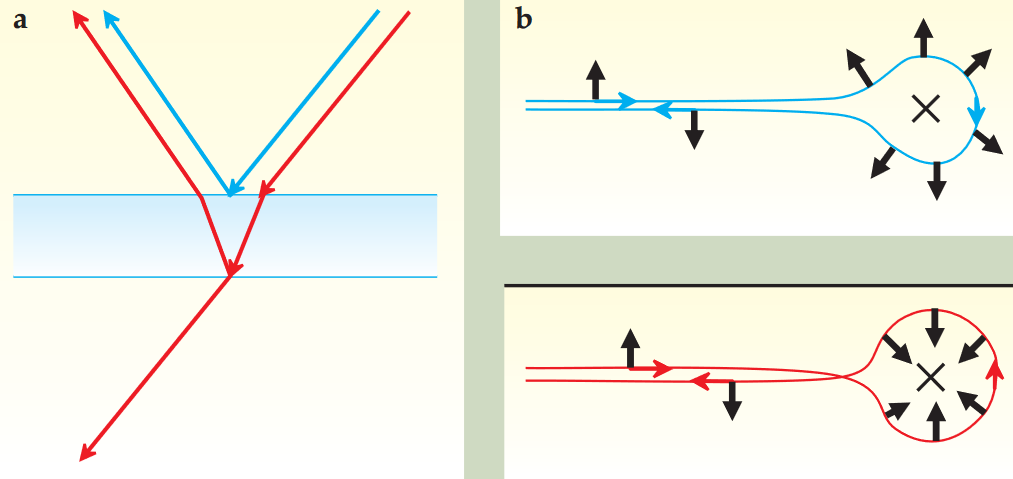
\includegraphics[scale = 0.7]{sections/visuel/lens.png}
    \caption{Analogy between an antireflection lens (A) and the interference phenomena (B) occuring in the QSH state to prevent backscattering on impurities represented by $X$ \cite{qi_quantum_2010}}
    \label{lens}
\end{figure*}



\begin{figure}[h!]
    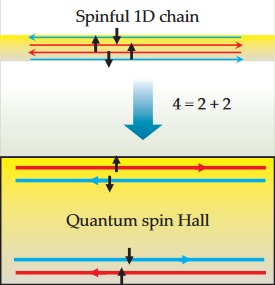
\includegraphics[scale = 0.7]{sections/visuel/spinful.png}
    \caption{Schematic representation of the conduction chanels in a spinlful quantum Hall system.}
    \label{spinful}
\end{figure}

% Talk about the fact that the states are topologicaly protected since their edge states survive the addition of impurities \cite{kane_this_2011}

%\section{\label{sec:berry_phase} Berry phase}
%Notion of holonomy in the phase of Bloch state transported in the Brillouin zone around a closed loop under the effect of the Berry connection.



%\section{\label{sec:z2_invariant} Invariants and Classification}
%\begin{enumerate}
%    \item Description of the $\mathbb{Z}_2$ invariant its relation with the Berry phase. 
%    \item Summary of the types of Topological insulator.
%    \item Bulk-boundary correspondence.\\[0.5cm]
%\end{enumerate}


\section{\label{sec:ti_exemples} HgTe/CdTe heterostructure}
As it was mentionned in sec. \ref{sec:QSH}, the QSH effect requiers strong spin-orbit coupling to occur. Kane and Mele initially proposed that the effect could be realised in graphene but the spin-orbit coupling of carbon is too weak \cite{cayssol_topological_2021}. The first observed topological insulator with QSH effect is a mercury telluride heterostructure consisting of a staking of thin \ch{HgTe} layers between \ch{Hg_xCd_{1-x}Te} \cite{kane_this_2011}. The Band structure of \ch{HgTe} and \ch{Hg_xCd_{1-x}Te} both contain a $\Gamma_6$ and $\Gamma_8$ band \cite{bernevig_topological_2013}. While the $\Gamma_6$ band is $s$-type, the $\Gamma_8$ band is $p$-type. A $s$-type (resp. $p$-type) is formed with the hybridization of $s$ (resp. $p$) orbitals with $0$ (resp. $1$) angular momentum quantum number \cite{girvin_modern_2019}. Adding spin leads to $1/2$ and $3/2$ respective total angular momentum quantum number for $\Gamma_6$ and $\Gamma_8$ bands \cite{bernevig_topological_2013}. 

If the thickness of the \ch{HgTe} layers is right, a spin Hall effect arises. \ch{Hg_xCd_{1-x}Te}

The signature of the appearence of a topologial phase with variation of the thickness is the band inversion \cite{bansil_colloquium_2016}. 

\begin{figure}[h!]
    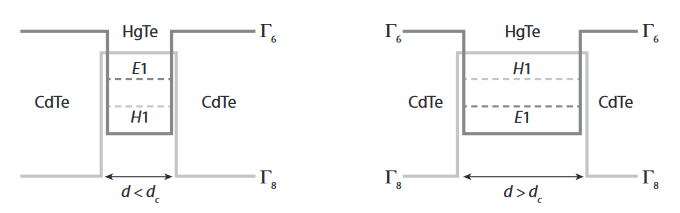
\includegraphics{sections/visuel/Hg}
    \caption{\cite{bernevig_topological_2013}}
\end{figure}

\section{\label{sec:concl} Conclusion}
\begin{enumerate}
    \item Opening on other topological systems (topological Superconductivity and charge pumps)\\[0.5cm]
\end{enumerate}
The study of topological insulators is a beautiful application of topology to solid-state physics. It gives profound insight on key properties of some material and some effects using what could've been considered abstract math. Some powerful concept such as the berry phase and Kramer’s theorem rapidly come into play. These concepts allow understanding otherwise very hard to understand yet important phenomena such has Hall effect. The mix of topological and solid-state physics physics howerver doesn't end there. There are other kinds of topological material such as topological \textit{superconductors}. Topological superconductivity, however, has been observed in far fewer materials. Such material still has important applications such as \textit{protected quantum computation}. \cite{nayak_evidence_2021} A lot of research of these materials will likely be done in the upcomming years.

\clearpage


\bibliographystyle{unsrt}
\bibliography{main.bib}


\end{document}
